\documentclass[a4paper,12pt]{article}
\usepackage{etex}
%%%%%%%%%%%%%%%%%%%%%%%%%%%%%%%%%%%%%%
% Babel language package
\usepackage[english,greek]{babel}
% Inputenc font encoding
\usepackage[utf8]{inputenc}
%%%%%%%%%%%%%%%%%%%%%%%%%%%%%%%%%%%%%%

%%%%% math packages %%%%%%%%%%%%%%%%%%
\usepackage{amsmath}
\usepackage{amssymb}
\usepackage{amsfonts}
\usepackage{amsthm}
\usepackage{proof}

\usepackage{physics}

%%%%%%% symbols packages %%%%%%%%%%%%%%
\usepackage{dsfont}
\usepackage{stmaryrd}
%%%%%%%%%%%%%%%%%%%%%%%%%%%%%%%%%%%%%%%


%%%%%% graphicx %%%%%%%%%%%%%%%%%%%%%%%
\usepackage{graphicx}
\usepackage{color}
%\usepackage{xypic}
\usepackage[all]{xy}
\usepackage{calc}
%%%%%%%%%%%%%%%%%%%%%%%%%%%%%%%%%%%%%%%

\usepackage{enumerate}

\usepackage{fancyhdr}
%%%%% header and footer rule %%%%%%%%%
\setlength{\headheight}{14pt}
\renewcommand{\headrulewidth}{0pt}
\renewcommand{\footrulewidth}{0pt}
\fancypagestyle{plain}{\fancyhf{}
\fancyhead{}
\lfoot{}
\rfoot{\small \thepage}}
\fancypagestyle{vangelis}{\fancyhf{}
\rhead{\small \leftmark}
\lhead{\small }
\lfoot{}
\rfoot{\small \thepage}}
%%%%%%%%%%%%%%%%%%%%%%%%%%%%%%%%%%%%%%%

\usepackage{hyperref}
\usepackage{url}
%%%%%%% hyperref settings %%%%%%%%%%%%
\hypersetup{pdfpagemode=UseOutlines,hidelinks,
bookmarksopen=true,
pdfdisplaydoctitle=true,
pdfstartview=Fit,
unicode=true,
pdfpagelayout=OneColumn,
}
%%%%%%%%%%%%%%%%%%%%%%%%%%%%%%%%%%%%%%



\usepackage{geometry}
\geometry{left=25.63mm,right=25.63mm,top=36.25mm,bottom=36.25mm,footskip=24.16mm,headsep=24.16mm}

%\usepackage[explicit]{titlesec}
%%%%%% titlesec settings %%%%%%%%%%%%%
%\titleformat{\chapter}[block]{\LARGE\sc\bfseries}{\thechapter.}{1ex}{#1}
%\titlespacing*{\chapter}{0cm}{0cm}{36pt}[0ex]
%\titleformat{\section}[block]{\Large\bfseries}{\thesection.}{1ex}{#1}
%\titlespacing*{\section}{0cm}{34.56pt}{17.28pt}[0ex]
%\titleformat{\subsection}[block]{\large\bfseries{\thesubsection.}{1ex}{#1}
%\titlespacing*{\subsection}{0pt}{28.80pt}{14.40pt}[0ex]
%%%%%%%%%%%%%%%%%%%%%%%%%%%%%%%%%%%%%%

%%%%%%%%% My Theorems %%%%%%%%%%%%%%%%%%
\newtheorem{thm}{Θεώρημα}[section]
\newtheorem{cor}[thm]{Πόρισμα}
\newtheorem{lem}[thm]{λήμμα}
\theoremstyle{definition}
\newtheorem{dfn}{Ορισμός}[section]
\newtheorem{dfns}[dfn]{Ορισμοί}
\theoremstyle{remark}
\newtheorem{remark}{Παρατήρηση}[section]
\newtheorem{remarks}[remark]{Παρατηρήσεις}
%%%%%%%%%%%%%%%%%%%%%%%%%%%%%%%%%%%%%%%




\input{definitions_ask.tex}
\usepackage{tikz}
\usetikzlibrary{calc}

\usetikzlibrary[shapes,angles,calc,arrows.meta,quotes,intersections]
\pgfdeclarelayer{fg}
\pgfdeclarelayer{bg}
\pgfsetlayers{bg,main,fg}
% \geometry{top=1cm}

\input{insbox}
\usepackage{wrapfig}

\pagestyle{vangelis}
\everymath{\displaystyle}
\setcounter{chapter}{1}

\begin{document}


\chapter*{Εξίσωση Ευθείας στο Χώρο}

Όπως είναι γνωστό, μια ευθεία στο επίπεδο, είναι δυνατόν να προσδιοριστεί, αν γνωρίζουμε
ένα σημείο της και έναν αριθμό που μας δείχνει την κλίση της. 
Στο χώρο, μια ευθεία μπορεί να προσδιοριστεί αν γνωρίζουμε ένα σημείο της
καθώς και το \textbf{διάνυσμα} που μας δείχνει την κατεύθυνσή της.


\section*{Ευθεία στο χώρο}


\begin{wrapfigure}{l}{0.28\linewidth}
  \begin{tikzpicture}[scale=0.7]
    \node  (0) at (0, 3) {};
    \node  (1) at (0, 0) {};
    \node  (2) at (-2, -1) {};
    \node  (3) at (3, 0) {};
    \node  (5) at (-1, 2) {};
    \node  (6) at (4, 3) {};
    \node[above] (e) at (6) {$\varepsilon$};
    \node  (7) at ($(5)!0.40!(6)$) {};
    \node  (8) at ($(5)!0.8!(6)$) {};
    \node  (u) at (2.375, 0.625) {};
    \node[above,yshift=-2pt,xshift=-5pt,Col2] (a) at (u) {$\mathbf{u}$};
    \draw[-latex,very thin] (1.center) node[left,yshift=3pt]{$O$} to (2.center) 
      node[left]{$x$};
    \draw[-latex,ultra thick,Col2] (1.center) to (u);
    \draw[-latex,very thin] (1.center) to (3.center) node[below]{$y$};
    \draw[-latex,very thin] (1.center) to (0.center) node[left]{$z$};
    \draw[very thick,Col1] (5.center) to (6.center);
    \draw[-latex] (1.center) to node[above left=-3pt]{$\mathbf{r_{0}}$} (7.center) 
      node[pin={[pin edge={black,latex-},Col2]93:\smaller$t=0$}]{}
      node[above,xshift=5pt]{\smaller$P_{0}$};
    \draw[-latex] (1.center) to node[right=5pt]{$\mathbf{r}$} (8.center) ;
    \draw[-latex,ultra thick,Col2] (7.center) to (8.center) node[above left] 
      {$t\mathbf{u}$};
    \node[above right] at (8) {\smaller$P$};
    \draw[fill] (7.center) circle (1.5pt); 
    \draw[fill] (8.center) circle (1.5pt); 
  \end{tikzpicture}
\end{wrapfigure}

Έστω $ \varepsilon $ ευθεία του χώρου που διέρχεται από το σημείο 
$ P_{0}(x_{0}, y_{0}, z_{0}) $ και είναι παράλληλη προς το διάνυσμα 
$ \mathbf{u} = a \mathbf{i} + b \mathbf{j} + c \mathbf{k} $. Τότε για το 
τυχαίο σημείο $ P(x,y,z) $ της ευθείας $ \varepsilon $, όπως φαίνεται στο σχήμα, ισχύει:
\begin{equation}\label{eq:vline}
  \mathbf{r} = \mathbf{r_{0}} + t \mathbf{u} \quad t \in \mathbb{R}
\end{equation}

Η εξίσωση~\eqref{eq:vline} λέγεται \textcolor{Col1}{διανυσματική παραμετρική} εξίσωση 
της ευθείας $ \varepsilon $  και σε πλήρη ανάπτυξη, παίρνει τη μορφή:
\begin{align*} 
  \mathbf{r}(t) = (x_{0}, y_{0}, z_{0}) + t (a, b, c) 
  = (x_{0} + t a, y_{0}+ t b, z_{0} + t c) 
\end{align*} 
ή ισοδύναμα, χρησιμοποιώντας τα μοναδιαία διανύσματα των αξόνων η παραπάνω εξίσωση
γράφεται
\[
  \boxed{\mathbf{r}(t) = (x_{0}+ t a) \mathbf{i} + (y_{0} + t b) \mathbf{j}+
  (z_{0}+ t c) \mathbf{k}} \quad t \in \mathbb{R} 
\]
Επομένως, αν $ \mathbf{r}(t) = (x(t), y(t), z(t)) $, έχουμε:

\begin{equation}\label{eq:pline}
  \boxed{
    \begin{matrix}
      x(t) = x_{0} + t a \\
      y(t) = y_{0} + t b \\
      z(t) = z_{0} + t c
    \end{matrix}
  } 
  \quad t \in \mathbb{R} 
\end{equation} 

Η εξισώσεις~\eqref{eq:pline} λέγονται \textcolor{Col1}{παραμετρικές εξισώσεις} της 
ευθείας $ \varepsilon $.

\begin{rem}
  Με απαλοιφή της παραμέτρου $t$ από τις εξισώσεις~\eqref{eq:pline} και αν 
  $ a, b, c \neq 0 $, παίρνουμε μια ακόμη ισοδύναμη έκφραση για την ευθεία που 
  διέρχεται από ένα σημείο $ P_{0}(x_{0}, y_{0}, z_{0}) $ και είναι παράλληλη προς το 
  διάνυσμα $ \mathbf{u} = (a,b,c) $:
  \begin{equation}\label{eq:fline}
    \boxed{\frac{x- x_{0}}{a} = \frac{y- y_{0}}{b} = \frac{z- z_{0}}{c}}
  \end{equation}
  Αν κάποια από τις συντεταγμένες του διανύσματος $ \mathbf{u} $ είναι 0, έστω $ a=0 $,
  τότε η εξίσωση~\eqref{eq:fline} παίρνει τη μορϕή:
  \[
    x = x_{0}, \quad \frac{y- y_{0}}{b} = \frac{z- z_{0}}{c}
  \]
\end{rem}


\begin{example}
  Να βρεθεί η εξίσωση της ευθείας που διέρχεται από το σημείο $ P_{0}(2,1,3) $ 
  και είναι παράλληλη στο διάνυσμα 
  $ \mathbf{u} = \mathbf{i}- 3 \mathbf{j}+2 \mathbf{k} $.
\end{example}
\begin{solution}
  Η εξίσωση της ευθείας σε διανυσματική μορϕή, είναι:
  \begin{align*}
    \mathbf{r}(t) &= \mathbf{r}_{0} + t \mathbf{u} = (2,1,3) + t(1,-3,2) \\
                  &= (2+t,1-3t,3+2t), \quad t \in \mathbb{R}
  \end{align*} 
  Άρα $ \mathbf{r}(t) = (2+t) \mathbf{i} + (1-3t) \mathbf{j} + (3+2t) \mathbf{k} $. 
  Επομένως οι παραμετρικές εξισώσεις της ευθείας, είναι:
  \[
    \left.
      \begin{matrix*}[l]
        x(t) = 2+t \\
        y(t) = 1-3t \\
        z(t) = 3+2t
      \end{matrix*} 
    \right\} \quad  t \in \mathbb{R} 
  \]
\end{solution}

\begin{example}\label{ex:line2}
  Να βρεθεί η εξίσωση της ευθείας που διέρχεται από τα σημεία $ Α(2,4,-3) $ και 
  $ B(3,-1,1) $. Σε ποιο σημείο, η ευθεία τέμνει το επίπεδο $ xy $; 
\end{example}
\begin{solution}
  Αρχικά, βρίσκουμε το διάνυσμα $ \vec{AB} $, που είναι παράλληλο με την ευθεία.
  \[ \vec{AB} = (3-2,-1,-4,1-(-3)) = (1,-5,4) \]
  Άρα η διανυσματική εξίσωση της ευθείας, είναι:
  \[
    \mathbf{r}(t) = (2,4,-3) + t(1,-5,4) = (2+t,4-5t,-3+4t)
  \] 
  ή ισοδύναμα, οι παραμετρικές της εξισώσεις, είναι:
  \begin{align*}
    x(t) &= 2+t \\
    y(t) &= 4-5t \\
    z(t) &= -3+4t
  \end{align*} 
  Η ευθεία, τέμνει το επίπεδο $ xy $, όταν $ z=0 $, δηλαδή όταν $ -3+4t=0
  \Leftrightarrow t = 3/4 $. Με αντικατάσταση, στις άλλες δύο παραμετρικές εξισώσεις, 
  βρίσκουμε:
  \[
    x = 2+ \frac{3}{4} = \frac{11}{4} \quad \text{και} \quad y = 4- 5\frac{3}{4} = 
    \frac{1}{4}  
  \]
  Επομένως, το σημείο στο οποίο η ευθεία, τέμνει το επίπεδο $ xy $, είναι το 
  $ (x,y) = (11/4,1/4) $.
\end{solution}

\begin{rem}
  Στη λύση του παραδείγματος~\ref{ex:line2}, θα μπορούσαμε να είχαμε χρησιμοποιήσει 
  τις συντεταγμένες του σημείου $ B $, αντί για αυτές του σημείου $A$, για την εξίσωση 
  της ευθείας, ή ακόμη και το διάνυσμα $ \vec{BA} $, αντί για το $ \vec{AB} $, που 
  είναι επίσης παράλληλο στην ευθεία. Τότε θα καταλήγαμε σε μια διαφορετική, αλλά 
  ισοδύναμη εξίσωση, που αναπαριστά την ίδια ευθεία. Επομένως, η αναπαράσταση, μιας 
  ευθείας, με τους τρόπους που περιγράψαμε παραπάνω, δεν είναι μοναδική.
\end{rem}
\begin{rem}
  Στο παράδειγμα~\ref{ex:line2}, παρατηρούμε ότι αν επιλέξουμε $ t=0 $, τότε οι 
  παραμετρικές εξισώσεις, μας δίνουν τις συντεταγμένες του σημείου $ A $, ενώ για 
  $ t=1 $, παίρνουμε το σημείο$ B $. Επομένως το ευθύγραμμο τμήμα $ AB $, 
  περιγράφεται από τις εξισώσεις:
  \[
    \left.
      \begin{matrix*}[l]
        x(t) &= 2+t \\
        y(t) &= 4-5t \\
        z(t) &= -3+4t
      \end{matrix*} 
    \right\} \quad  t \in [0,1]
  \]
\end{rem}


\section*{Ευθύγραμμο Τμήμα στο χώρο}

\begin{wrapfigure}{l}{0.28\linewidth}
  \begin{tikzpicture}[scale=0.7]
    \node  (0) at (0, 3) {};
    \node  (1) at (0, 0) {};
    \node  (2) at (-2, -1) {};
    \node  (3) at (3, 0) {};
    \node  (5) at (-0.75, 2) [pin={[pin
      edge={black,latex-},Col2]115:\smaller$t=0$}] {};
    \node  (6) at (3.5, 1) [pin={[pin
      edge={black,latex-},Col2]93:\smaller$t=1$}] {};
    \node[above,xshift=2pt] (a) at (5) {$A$};
    \node[above,xshift=5pt] (b) at (6) {$B$};
    \draw[-latex,very thin] (1.center) node[left,yshift=3pt]{$O$} to (2.center) 
      node[left]{$x$};
    \draw[-latex,very thin] (1.center) to (3.center) node[below]{$y$};
    \draw[-latex,very thin] (1.center) to (0.center) node[left]{$z$};
    \draw[-latex] (1.center) to node[left]{$\mathbf{r_{A}}$} (5.center);
    \draw[-latex] (1.center) to node[above]{$\mathbf{r_{B}}$} (6.center);
    \draw[fill,Col2] (5.center) circle (2pt); 
    \draw[fill,Col2] (6.center) circle (2pt); 
    \draw[very thick,->,Col1] (5.center) to ($(5)!0.5!(6)$);
    \draw[ultra thick,Col1] (5.center) to (6.center);
  \end{tikzpicture}
\end{wrapfigure}

Γενικά η διανυσματική παραμετρική εξίσωση του \textcolor{Col1}{ευθύγραμμου τμήματος} 
$ AB $, όπου $ \mathbf{r}_{A} $ και $ \mathbf{r}_{B} $ είναι τα διανύσματα θέσης, 
αντίστοιχα, των σημείων $ A(x_{A},y_{A},z_{A}) $ και $B(x_{B},y_{B},z_{B})$, είναι 
\[
  \boxed{\mathbf{r} = \mathbf{r}_{A} + t(\mathbf{r}_{B}- \mathbf{r}_{A})} 
  \quad \text{ή} \quad \boxed{\mathbf{r} = (1-t) \mathbf{r}_{A} + t \mathbf{r}_{B}}, 
  \quad t \in [0,1]
\] 
και οι αντίστοιχες παραμετρικές εξισώσεις, είναι:
\[
  \boxed{\left.
      \begin{matrix*}[l]
        x(t) = x_{A} + t(x_{B}-x_{A}) \\
        y(t) = y_{A} + t(y_{B}-y_{A}) \\
        z(t) = z_{A} + t(z_{B}-z_{A}) 
      \end{matrix*} 
  \right\}} \quad \text{ή} \quad  
  \boxed{\left.
      \begin{matrix*}[l]
        x(t) = (1-t)x_{A} + tx_{B} \\
        y(t) = (1-t)y_{A} + ty_{B} \\
        z(t) = (1-t)z_{A} + tz_{B} 
      \end{matrix*} 
  \right\}} \quad t \in [0,1]
\]

\begin{example}
  Οι παραμετρικές εξισώσεις του ευθυγράμμου τμήματος $ AB $, που ενώνει τα σημεία 
  $ A(3,-2,1) $ και $ B(-2,1,0) $, είναι:
  \[
    \left.
      \begin{matrix*}[l]
        x(t) = 3+t(-2-3) \\
        y(t) = -2+t(1-(-2)) \\
        z(t) = 1+t(0-1)
      \end{matrix*} 
    \right\} \Leftrightarrow 
    \left.
      \begin{matrix*}[l]
        x(t) = 3-5t \\
        y(t) = -2+3t \\
        z(t) = 1-1t
      \end{matrix*} 
    \right\} \quad t \in [0,1]
  \] 
\end{example}


\section*{Ευθύγραμμη Κίνηση}

Αν υποθέσουμε ότι, το σημείο $ P(x_{0}, y_{0}, z_{0}) $, είναι η αρχική θέση στο 
χώρο, ενός υλικού σημείου, το οποίο κινείται ευθύγραμμα και ομαλά (με σταθερή ταχύτητα) 
προς την κατεύθυνση του διανύσματος $ \mathbf{u} $, τότε η εξίσωση~\eqref{eq:vline}, 
αν την ξαναγράψουμε ως
\[
  \boxed{\mathbf{r} = \mathbf{r}_{0} + t \norm{\mathbf{u}}
  \frac{\mathbf{u}}{\norm{\mathbf{u}}}}
\]
παριστάνει την \textbf{εξίσωση κίνησης} του υλικού σημείου, αφού η ποσότητα 
$ t \norm{\mathbf{u}} $ παριστάνει την απόσταση που διανύει το σημείο, σε χρόνο $t$, 
αν κινείται με ταχύτητα $ \norm{\mathbf{u}} $ προς την κατεύθυνση του διανύσματος 
$ \mathbf{u}/ \norm{\mathbf{u}} $.

\begin{example}
  Ένα ελικόπτερο, που βρίσκεται αρχικά στην αρχή των αξόνων, κινείται προς την
  κατεύθυνση του σημείου $P(1,1,1) $ με ταχύτητα $ \SI{60}{m/s} $. Ποια, θα είναι 
  η θέση του ελικοπτέρου, μετά από 10 δευτερόλεπτα;
\end{example}
\begin{solution}
  Αρχικά, βρίσκουμε το διάνυσμα $ \mathbf{u} = \vec{PO} $, που μας προσδιορίζει την
  κατεύθυνση του ελικοπτέρου. Είναι
  \[ \mathbf{u} = (1-0,1-0,1-0) = (1,1,1) \]
  Άρα το μοναδιαίο διάνυσμα είναι $ \mathbf{\widehat{u}} =
  \frac{\mathbf{u}}{\norm{\mathbf{u}}} = \frac{1}{\sqrt{3}} (1,1,1) =
  \left(\frac{1}{\sqrt{3}} , \frac{1}{\sqrt{3}} , \frac{1}{\sqrt{3}}\right) $. Η εξίσωση
  κίνησης, είναι:
  \[
    \mathbf{r}(t) = \mathbf{0} + t 60 \mathbf{\widehat{u}} = (0,0,0) + 60t 
    \left(\frac{1}{\sqrt{3}} , \frac{1}{\sqrt{3}} , \frac{1}{\sqrt{3}}\right) = 
    20 \sqrt{3} t (1,1,1).
  \] 
  Άρα, για $ t= \SI{10}{s} $ η θέση του ελικοπτέρου, θα είναι $ \mathbf{r}(10) = 200
  \sqrt{3} (1,1,1) = (200 \sqrt{3} , 200 \sqrt{3} , 200 \sqrt{3}) $. 
\end{solution}

\chapter*{Εξίσωση Επιπέδου στο Χώρο}



Ένα επίπεδο, μπορεί να προσδιορισθεί, αν γνωρίζουμε ένα σημείο του, και ένα 
διάνυσμα που είναι κάθετο σε αυτό, και το οποίο μας δείχνει τον προσανατολισμό του 
επιπέδου στο χώρο.

\section*{Επίπεδο στο χώρο}

\begin{wrapfigure}{l}{0.34\linewidth}
  \begin{tikzpicture}[scale=0.7]
  %axes
  \coordinate  (0) at (0, 0) [label=left:$O$] {};
  \node  (x) at (-2, -1)[label={[left]:$x$}] {};
  \node  (y) at (4, 0) [label={[below right]:$y$}]{};
  \node  (z) at (0, 4) [label={[below left]:$z$}] {};
  \begin{pgfonlayer}{bg}
    \path[name path=z,-latex] (0.center) to (z.center);
    \path[name path=y,-latex] (0.center) to (y.center);
    \draw[-latex] (0.center) to (x.center);
  \end{pgfonlayer}
  \coordinate  (c) at (2.25, 3.75) {};
  \coordinate  (b) at (5.75, 1.75) {};
  \coordinate  (d) at (-1.25, 1.5) {};
  \coordinate  (a) at (2.25, -0.5) {};
  \coordinate  (po) at (3, 1) {};
  \coordinate  (p) at (1.75, 1.80) {};
  \begin{pgfonlayer}{fg}
  \end{pgfonlayer}
  \node[above right,xshift=3pt] (PO) at (po) {\smaller$P_{0}$};
  \node[above] (P) at (p) {\smaller$P(x,y,z)$};
  \begin{pgfonlayer}{fg}
    \draw[ultra thick,-latex,Col2] (po.center) to (p.center);
    \draw[ultra thick,-latex,Col1] (po.center) to (4,3.5) node[right] (n) {$\mathbf{n}$};
    \draw[fill] (p) circle (1.5pt);
    \draw[fill] (po) circle (1.5pt);
  \end{pgfonlayer}
  \begin{pgfonlayer}{bg}
    \path[name path=p] (0.center) to node[above left] {$\mathbf{r}$} (p.center);
    \path[name path=po] (0.center) to node[below right] {$\mathbf{r_{0}}$} (po.center);
  \end{pgfonlayer}
  %make the right angle
  \coordinate (an1) at ($(po)!7pt!(n)$) ;
  \coordinate (an2) at ($(po)!7pt!(p)$) ;
  \draw (an1) -- ($(an1)+(-0.10,0.3,0.35)$) -- (an2); 
  \draw[name path=plane,fill,blue!50,opacity=0.4] (a) -- (b) -- (c) -- (d) -- (a) ;
  \coordinate [name intersections={of=p and plane, by=1}];
  \coordinate [name intersections={of=po and plane, by=2}];
  \coordinate [name intersections={of=z and plane, by={z2,z1}}];
  \coordinate [name intersections={of=y and plane, by={y2,y1}}];
  \begin{pgfonlayer}{bg}
    \draw (0) -- (z1) ;
    \draw[dashed] (z1) -- (z2) ;
    \draw[-latex] (z2) -- (z) ;
    \draw (0) -- (y1) ;
    \draw[dashed] (y1) -- (y2) ;
    \draw[-latex] (y2) -- (y) ;
    \draw (0) to (1);
    \draw (0) to (2);
  \end{pgfonlayer}
  \begin{pgfonlayer}{bg}
    \draw[dashed,-latex] (1) to (p);
    \draw[dashed,-latex] (2) to (po);
  \end{pgfonlayer}
\end{tikzpicture}
\end{wrapfigure}
Έστω $ \Pi $ επίπεδο του χώρου που διέρχεται από το σημείο 
$ P_{0}(x_{0}, y_{0}, z_{0}) $ 
και έστω $ \vec{n} = a \mathbf{i} + b \mathbf{j} + c \mathbf{k} $, ένα διάνυσμα κάθετο 
στο επίπεδο. Τότε για το τυχαίο σημείο $ P(x,y,z) $ του επιπέδου $ \Pi $, όπως φαίνεται 
στο σχήμα, ισχύει ότι 
\begin{equation}\label{eq:vplane}
  \vec{n} \cdot (\mathbf{r} - \mathbf{r}_{0}) = 0
\end{equation} 
αφού το διάνυσμα $ \vec{n} $, είναι κάθετο και σε όλα τα διανύσματα του επιπέδου, άρα 
και στο διάνυσμα $ \vec{P_{0}P} $. 
Η εξίσωση~\eqref{eq:vplane} λέγεται \textcolor{Col1}{διανυσματική} εξίσωση του 
επιπέδου $ \Pi $ και σε πλήρη ανάπτυξη, παίρνει τη μορφή:
\begin{equation*}
  (a,b,c) \cdot (x- x_{0}, y- y_{0}, z- z_{0}) = 0 
\end{equation*} 
ή ισοδύναμα, υπολογίζοντας το εσωτερικό γινόμενο, έχουμε
\begin{equation}
  \boxed{a(x- x_{0}) + b(y- y_{0}) + c(z- z_{0}) = 0}
\end{equation}
η οποία, μετά από πράξεις, γράφεται στην πιο απλή μορφή:
$ ax+by+cz=d $, όπου $ d=a x_{0}+ b y_{0}+cz_{0} $.



\begin{example}
  Βρείτε την εξίσωση του επιπέδου, που διέρχεται από το σημείο $ P_{0}(2,4,-1) $, με 
  κάθετο διάνυσμα $ \vec{n} = 2 \mathbf{i} + 3 \mathbf{j} + 4 \mathbf{k} $. Να βρείτε 
  τα σημεία τομής τους επιπέδου με τους άξονες, και να το σχεδιάσετε.
\end{example}
\begin{solution}
  Η εξίσωση του επιπέδου, είναι:
  \[
    2(x-2)+3(y-4)+4(z-(-1)) = 0 \Leftrightarrow 2x+3y+4z=12
  \]
  Για να βρούμε τα σημεία τομής του επιπέδου με τους άξονες, έχουμε:
  \InsertBoxR{1}{\parbox[b][1.5\baselineskip][c]{0.33\textwidth}
    {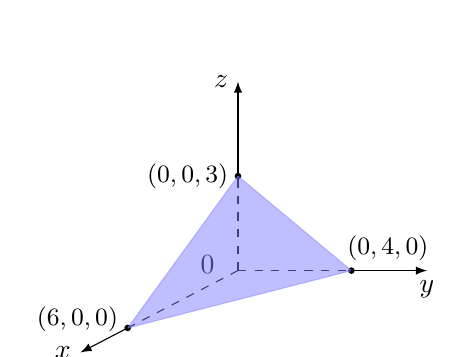
\begin{tikzpicture}[scale=0.8]
    \begin{pgfonlayer}{bg}
      \coordinate (o) at (0,0) ;
      \node at (o) [left=5pt,yshift=2pt] {$0$} ;
      \coordinate (z) at (0,3) ;
      \node at (z) [left] {$z$} ;
      \coordinate (y) at (3,0) ;
      \node at (y) [below] {$y$} ;
      \coordinate (x) at (-2.5,-1.3) ;
      \node at (x) [left] {$x$} ;
      \coordinate (a) at ($(o)!0.7!(x)$) ;
      \coordinate (b) at ($(o)!0.6!(y)$) ;
      \coordinate (c) at ($(o)!0.5!(z)$) ;
      \draw[dashed] (o) to (a);
      \draw[dashed] (o) to (b);
      \draw[dashed] (o) to (c);
      \fill (a) circle (1.5pt) ;
      \fill (b) circle (1.5pt) ;
      \fill (c) circle (1.5pt) ;
    \end{pgfonlayer}
    \draw[fill,blue!50,opacity=0.5] (a) to (b) to (c) to (a) ;
    \draw[-latex] (a) to (x);
    \draw[-latex] (b) to (y);
    \draw[-latex] (c) to (z);
    \node at (a) [left,yshift=3pt] {\small$(6,0,0)$} ;
    \node at (b) [above right,xshift=-5pt] {\small$(0,4,0)$} ;
    \node at (c) [left] {\small$(0,0,3)$} ;
  \end{tikzpicture}}}
  \begin{myitemize}
    \item Για τον άξονα $z$, θέτουμε $ x=y=0 $ και βρίσκουμε $ z=3 $.
    \item Για τον άξονα $x$, θέτουμε $ y=z=0 $ και βρίσκουμε $ x=6 $.
    \item Για τον άξονα $y$, θέτουμε $ x=z=0 $ και βρίσκουμε $ y=4 $.
  \end{myitemize}
  Με τη βοήθεια αυτών των σημείων, μπορούμε να σχεδιάσουμε, εύκολα, το τμήμα του 
  επιπέδου, που βρίσκεται στο 1ο ογδοημόριο, όπως φαίνεται στο σχήμα.
\end{solution}

\begin{example}
  Βρείτε την εξίσωση του επιπέδου, που διέρχεται από τα σημεία 
  $ P(1,3,2) $, $ Q(3,-1,6) $ και $R(5,2,0) $.
\end{example}
\begin{solution}
  Βρίσκουμε τα διανύσματα $ \vec{PQ} $ και $ \vec{PR} $, που περιέχονται στο επίπεδο.
  \begin{align*}
    \vec{PQ} &= (3-1,-1-3,6-2) = (2,-4,4) \\
    \vec{PR} &= (5-1,2-3,0-2) = (4,-1,-2)
  \end{align*} 
  Το διάνυσμα $ \vec{PQ} \times \vec{PR} $ είναι κάθετο στα δύο διανύσματα, και άρα 
  κάθετο και στο επίπεδο. Οπότε
  \[
    \vec{PQ} \times \vec{PR} = 
    \begin{vmatrix*}[r]
      \mathbf{i} & \mathbf{j} & \mathbf{k} \\
      2 & -4 & 4 \\
      4 & -1 & -2
    \end{vmatrix*} = 12 \mathbf{i} + 20 \mathbf{j} + 14 \mathbf{k}
  \] 
  Άρα η εξίσωση του επιπέδου, θα είναι 
  \[
    12(x-1) + 20(y-3) + 14(z-2) = 0 \Leftrightarrow 6x+10y+7z=50
  \]
\end{solution}


\begin{example}
  Βρείτε το σημείο, στο οποίο η ευθεία με παραμετρικές εξισώσεις $ x=2+3t $, $ y=-4t
  $ και $ z=5+t $ τέμνει το επίπεδο $ 4x+5y-2z=18 $.
\end{example}
\begin{solution}
  Για να βρούμε τα σημεία τομής της ευθείας και του επιπέδου, λύνουμε το σύστημα των 
  εξισώσεών τους, οπότε με αντικατάσταση των παραμετρικών εξισώσεων της ευθείας, 
  στην εξίσωση του επιπέδου, έχουμε:
  \[
    4(2+3t) + 5(-4t) -2(5+t) = 18 \Leftrightarrow -10t=20 \Leftrightarrow t=-2 
  \] 
  Με αντικατάσταση $ t=-2 $ στις παραμετρικές εξισώσεις της ευθείας, εύκολα 
  βρίσκουμε ότι:
  \[
    x=-4 \quad y=8 \quad z=3
  \] 
  Επομένως το σημείο τομής της ευθείας και του επιπέδου, είναι $ (x,y,z) = (-4,8,3) $.
\end{solution}

\begin{example}
  Να βρεθεί η εξίσωση της ευθείας, που διέρχεται από το σημείο $ P(0,-7,0) $ 
  και είναι κάθετη στο επίπεδο $ x+2y+2z=13 $.
\end{example}
\begin{solution}
  Ένα διάνυσμα κάθετο στο επίπεδο, και επομένως παράλληλο προς την ζητούμενη ευθεία, 
  είναι το $ \vec{n} = (1,2,2) $. Άρα η εξίσωση της ευθείας, είναι:
  \[
    \mathbf{r} = (0,-7,0) + t(1,2,2,) = (t, -7+2t, 2t) 
  \]
  Άρα οι παραμετρικές εξισώσεις της ευθείας, είναι 
  \[
    \left. 
      \begin{matrix*}[l]
        x(t)=t \\
        y(t)=-7+2t \\
        z(t)=2t
      \end{matrix*} 
    \right\} \quad t \in \mathbb{R}
  \] 
\end{solution}

\begin{example}
  Να βρείτε το σημείο τομής των ευθειών, $ \varepsilon _{1}: x=t, \; y=-t+2, \;
  z=t+1$ και $ \varepsilon _{2}; x=2s+2, \; y=s+3, \; z=5s+6 $, και στη συνέχεια να 
  βρείτε την εξίσωση του επιπέδου, που ορίζουν αυτές οι δύο ευθείες.
\end{example}
\begin{solution}
  Για να βρούμε το σημείο τομής των δύο ευθειών, λύνουμε το σύστημα των εξισώσεών τους.
  \[
    \left.
      \begin{matrix}
        x=t=2s+2 \\
        y=-t+2=s+3
      \end{matrix} 
    \right\} \Leftrightarrow 
    \left.
      \begin{matrix}
        t-2s=2 \\
        -t-s=1
      \end{matrix} 
    \right\} \Leftrightarrow s=-1 \quad \text{και} \quad t=0
  \] 
  Οπότε $ z=t+1=5s+6 $ και για $ s=-1 $ και $ t=0 $, έχουμε ότι $ 0+1=5(-1)+6
  \Leftrightarrow 1 = 1 $, δηλαδή ικανοποιείται και η 3η εξίσωση. Άρα οι δύο 
  ευθείες, τέμνονται για $ s=-1, \; t=0 $, στο σημείο με $ x=0, \; y=2, \; z=1 $, 
  δηλαδή $ P(0,2,1) $.

  Ένα διάνυσμα κάθετο στις δύο ευθείες, επομένως και στο επίπεδο που ορίζουν είναι, το
  \[
    \vec{n_{1}} \times \vec{n_{2}} = 
    \begin{vmatrix*}[r]
      \mathbf{i} & \mathbf{j} & \mathbf{k} \\
      1 & -1 & 1 \\
      2 & 1 & 5 
    \end{vmatrix*} = -6 \mathbf{i}-3 \mathbf{j}+3 \mathbf{k}
  \]  
  Άρα η εξίσωση του ζητούμενου επιπέδου, είναι 
  \[
    -6(x-0)+(-3)(y-2)+3(z-1)=0 \Leftrightarrow 6x+3y-3z=3 
  \]
\end{solution}


\section*{Γωνία δύο επιπέδων}

  \InsertBoxR{0}{\parbox[b][3\baselineskip][c]{0.30\textwidth}
    {\begin{tikzpicture}[scale=0.8]
        \node (o) at (0, 0) {};
        \node (a) at (4, 0) {};
        \node (b) at (6, 1) {};
        \node (c) at (2, 1) {};
        \node (d) at (5.5, 2.25) {} ;
        \node (e) at (1.5, 2.25) {} ;
        \node (v1) at (3, 0.5) {};
        \node["$\mathbf{n_{1}}$"] (v2) at (3, 3) {};
        \node (d1) at (3, 1.25) {};
        \node["$\mathbf{n_{2}}$"] (d2) at (1.5, 3) {};
        \begin{pgfonlayer}{fg}
          \draw[-latex] (d1.center) to (v2.center);
          \draw[-latex] (d1.center) to (d2.center);
          \draw[fill] (d1) circle (.5pt) ;
        \end{pgfonlayer}
        \begin{pgfonlayer}{bg}
          \path[fill=Col1!50] (o.center) to (a.center) to (b.center) to 
            (intersection of b--c and a--d) to[every to={draw=red,dashed}] (c.center) -- 
            cycle   ;
          \draw[dashed] (v1.center) to (d1.center);
          \coordinate (k) at ($(v1)+(.2,.2)$) ;
          \draw (v1|-k) -- (k) -- (v1-|k) ;
          \node[xshift=-18pt,yshift=-3pt] at (b.200) {\smaller$\Pi_{1}$} ;
          \path pic[draw,angle radius=13pt,"$\theta$",angle eccentricity=1.5] 
            {angle=b--a--d};
        \end{pgfonlayer}
        \begin{pgfonlayer}{fg}
          \path pic[draw,angle radius=10pt,"$\theta$",angle eccentricity=1.5] 
            {angle=v2--d1--d2};
          \coordinate (l) at ($(d1)!0.1!(d2)$) ;
          \draw (l) -- ++ (-.15,-.15) -- ++(.15,-.15) ;
        \end{pgfonlayer}
        \path[fill=blue!50,opacity=0.5] (o.center) to (a.center) to (d.center) to 
          (e.center) -- cycle   ;
        \node[xshift=-10pt,yshift=-5pt] at (d.210) {\smaller$\Pi_{2}$} ;
  \end{tikzpicture}}}

  Δυο επίπεδα, είναι \textcolor{Col1}{παράλληλα}, αν και μόνον αν τα κάθετα διανύσματα 
  τους, είναι παράλληλα. Για παράδειγμα τα επίπεδα $ x+2y-3z=4 $ και $ 2x+4y-6z=3 $ 
  είναι παράλληλα, γιατί τα κάθετα διανύσματα $ \vec{n_{1}} = (1,2,-3) $ και 
  $ \vec{n_{2}} = (2,4,-6) $ είναι επίσης παράλληλα, αφού 
  $ \vec{n_{2}} = 2 \vec{n_{1}} $. Αν δύο επίπεδα, δεν είναι παράλληλα, τότε τέμνονται 
  σε μία ευθεία, και η \textcolor{Col1}{γωνία} μεταξύ τους ορίζεται να είναι η 
  \textbf{οξεία} γωνία που σχηματίζουν τα κάθετα διανύσματά τους.

\begin{rem}
  Σύμφωνα με την παραπάνω παρατήρηση το διάνυσμα 
  $ \vec{n_{1}} \times \vec{n_{2}} $ είναι παράλληλο προς τα δύο επίπεδα, με κάθετα 
  διανύσματα τα $ \vec{n_{1}} $ και $ \vec{n_{2}} $. Επομένως, το διάνυσμα αυτό 
  θα είναι παράλληλο και προς την ευθεία, που αποτελείται από τα σημεία τομής τους.
\end{rem}

\begin{example}
  Βρείτε τη γωνία που σχηματίζουν τα επίπεδα $ x+y+z=1 $ και $ x-2y+3z=1 $ και 
  στη συνέχεια, βρείτε την εξίσωση της ευθείας που αποτελείται από τα σημεία τομής 
  των δύο επιπέδων.
\end{example}
\begin{solution}
  Τα κάθετα διανύσματα των δύο επιπέδων είναι:
  \[
    \vec{n_{1}} = (1,1,1) \quad \text{και} \quad \vec{n_{2}} = (1,-2,3) 
  \]
  και η γωνία που σχηματίζουν δίνεται από την σχέση:
  \[
    \cos{\theta} = \frac{\vec{n_{1}} \cdot \vec{n_{2}}}{\norm{\vec{n_{1}}}
    \norm{\vec{n_{2}}}} = \frac{1+(-2)+3}{\sqrt{3}\cdot \sqrt{14}} =
    \frac{2}{\sqrt{42}} \Rightarrow \theta = \arccos(\frac{2}{\sqrt{42}}) \approx 
    \SI{72}{\degree} 
  \] 
  Για την εξίσωση της ευθείας, χρειαζόμαστε ένα σημείο της, και ένα διάνυσμα 
  παράλληλό της. Μπορούμε να βρούμε το σημείο στο οποίο η ευθεία τέμνει το επίπεδο 
  $ xy $, θέτοντας $ z=0 $ στις εξισώσεις των δύο επιπέδων. Πράγματι 
  \[
    \left.
      \begin{matrix}
        x+y=1 \\
        x-2y=3
      \end{matrix} 
    \right\} \Leftrightarrow 
    \left.
      \begin{matrix}
        x=1 \\
        y=0
      \end{matrix} 
    \right\} 
  \] 
  Άρα, ένα σημείο της ευθείας, είναι το $ (x,y,z) = (1,0,0) $.
  Ένα διάνυσμα παράλληλο στην ευθεία, είναι το $ \vec{n_{1}} \times \vec{n_{2}} $, 
  όπου
  \[
    \vec{n_{1}} \times \vec{n_{2}} = 
    \begin{vmatrix*}[r]
      \mathbf{i} & \mathbf{j} & \mathbf{k} \\
      1 & 1 & 1 \\
      1 & -2 & 3
    \end{vmatrix*} = 5 \mathbf{i}- 2 \mathbf{j}+ 3 \mathbf{k} 
  \] 
  Άρα η διανυσματική εξίσωση της ευθείας είναι 
  $ \mathbf{r}(t) = (1,0,0) + t(5,-2,3) $, με παραμετρικές εξισώσεις:
  \[
    \left.
      \begin{matrix*}[l]
        x(t) = 1+5t \\
        y(t) = -2t \\
        z(t) = 3t
      \end{matrix*} 
    \right\} \quad t \in \mathbb{R}
  \]
\end{solution}



\end{document}
